\section{滤波}
相关命令:\nameref{cmd:bandpass}、\nameref{cmd:lowpass}、\nameref{cmd:highpass}、
\nameref{cmd:bandrej}

几乎所有的数据分析都需要将数据限制在一定的频率范围内,对数据做低通、高通或带通滤波
很有必要。

\begin{figure}[H]
\centering
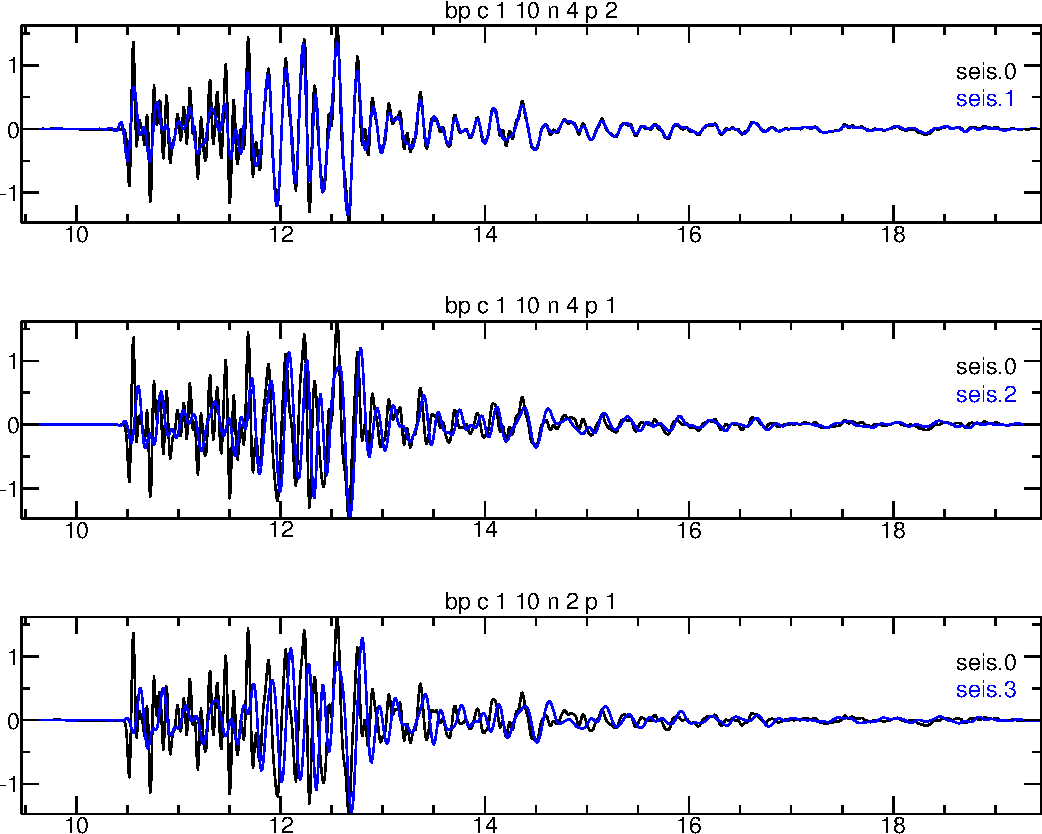
\includegraphics[width=0.8\textwidth]{filter}
\caption{带通滤波效果}
\label{fig:filter}
\end{figure}

\begin{SACCode}
SAC> fg seis
SAC> rmean; rtr; taper
SAC> w seis
SAC> bp c 1 10 n 4 p 2  // 4阶2通道butterworth带通滤波
SAC> r seis
SAC> bp c 1 10 n 4 p 1  // 4阶1通道butterworth带通滤波
SAC> r seis
SAC> bp c 1 10 n 2 p 1  // 2阶1通道butterworth带通滤波
\end{SACCode}

图~\ref{fig:filter}~中分别给出了使用三种滤波器之后的波形与原波形的对比图。
